%\documentclass[first,firstsupp,handout,compress,notes,navigation]{ETHclass} 
%\documentclass[first,firstsupp,handout,lastsupp]{ETHclass} 
\documentclass[first,firstsupp,lastsupp,handout,last,hyperref,table]{ETHclass} 
%\documentclass[first,firstsupp]{ETHclass}
\usepackage{etex}
\usepackage[utf8]{inputenc}
\usepackage[T1]{fontenc}
\usepackage{adjustbox}
\usepackage{amsmath}
\usepackage{amssymb}
\usepackage{animate}
\usepackage{booktabs}
\usepackage{charter}
\usepackage{etoolbox}
\usepackage{ifthen}
\usepackage{longtable}
\usepackage{mathrsfs}
\usepackage{multicol}
\usepackage{pgf}
\usepackage{ragged2e}
\usepackage{standalone}
\usepackage[caption=false]{subfig}
\usepackage{tabularx}
\usepackage{tikz}
\usepackage{verbatim}
\usepackage{xcolor}
\usepackage{hyperref}




\setbeamertemplate{navigation symbols}{}
\usetikzlibrary{arrows,decorations.pathreplacing,positioning,shapes,shadows}

%\usepackage[style=numeric-comp]{biblatex}

%\usepackage{lipsum}

%\usetikzlibrary{fit}
\usetikzlibrary{arrows}
\usetikzlibrary{trees}

% Options for beamer:
%
% 9,10,11,12,13,14,17pt  Fontsizes
% 
% compress: navigation bar becomes smaller
% t       : place contents of frames on top (alternative: b,c)
% handout : handoutversion
% notes   : show notes
% notes=onlyslideswithnotes
%
%hyperref={bookmarksopen,bookmarksnumbered} : Needed for menues in
%                                             acrobat. Also need
%                                             pdftex as option or 
%                                             compile with
% pdflatex '\PassOptionsToPackage{pdftex,bookmarksopen,bookmarksnumbered}{hyperref} \input{file}'

%\usepackage{beamerseminar}
%\usepackage[accumulated]{beamerseminar}
                                % remove ``accumulated'' option
                                % for original behaviour
%\usepackage{beamerbasenotes}
%\setbeamertemplate{note page}[plain] 
%\setbeameroption{notes on second screen}

%\setbeamertemplate{note page}[plain] 
\setbeamertemplate{note page}{\ \\[.3cm]
\textbf{\color{blue}Notes:}\\%[0.1cm]
{\footnotesize %\tiny
\insertnote}}
%\setbeameroption{notes on second screen}


%\setbeamertemplate{navigation symbols}{} % suppresses all navigation symbols:
 \setbeamertemplate{navigation symbols}[horizontal] % Organizes the navigation symbols horizontally.
% \setbeamertemplate{navigation symbols}[vertical] % Organizes the navigation symbols vertically.
% \setbeamertemplate{navigation symbols}[only frame symbol] % Shows only the navigational symbol for navigating frames.

\setlayoutscale{0.5}
\setparametertextfont{\scriptsize}
\setlabelfont{\scriptsize}

% \useoutertheme[subsection=false]{miniframes}
% \usepackage{etoolbox}
% \makeatletter
% \patchcmd{\slideentry}{\advance\beamer@xpos by1\relax}{}{}{}
% \def\beamer@subsectionentry#1#2#3#4#5{\advance\beamer@xpos by1\relax}%
% \makeatother

% \makeatletter
%     \newenvironment{withoutheadline}{
%        \setbeamertemplate{headline}{%
% \vspace{15pt}
% }
%     }{}
% \makeatother

\makeatletter
    \newenvironment{withoutheadline}{
         \setbeamertemplate{headline}{%
\vspace{35pt}
}
        %\def\beamer@entrycode{\vspace*{-1.5\headheight}}
    }{}
\makeatother

\newcommand{\Cross}{$\mathbin{\tikz [x=1.4ex,y=1.4ex,line width=.2ex, red] \draw (0,0) -- (1,1) (0,1) -- (1,0);}$}%

\newcommand{\Checkmark}{$\color{green}\checkmark$}

\setbeamerfont{subsection in toc}{size=\tiny}

\makeatletter
\patchcmd{\beamer@sectionintoc}
  {\vfill}
  {\vskip1.5\itemsep}
  {}
  {}
\makeatother  

\setbeamertemplate{frametitle continuation}{}

\setbeamertemplate{bibliography entry title}{}
\setbeamertemplate{bibliography entry author}{}
\setbeamertemplate{bibliography entry location}{}
\setbeamertemplate{bibliography entry note}{}

\setbeamercolor*{bibliography entry title}{fg=black}
\setbeamercolor*{bibliography entry author}{fg=black}
\setbeamercolor*{bibliography entry location}{fg=black}
\setbeamercolor*{bibliography entry note}{fg=black}
% and kill the abominable icon
%\setbeamertemplate{bibliography item}{\color{forestgreen}$\blacktriangleright$}
\setbeamertemplate{bibliography item}{\insertbiblabel}
%\setbeamertemplate{bibliography item}{\theenumiv}

\newcommand{\highlightred}[1]{%
  \colorbox{red!50}{$\displaystyle#1$}}
  
\newcommand{\highlightyellow}[1]{%
  \colorbox{yellow!50}{$\displaystyle#1$}}
  
\newcommand{\highlightgreen}[1]{%
  \colorbox{green!50}{$\displaystyle#1$}}

\AtBeginSection[]{
  \begin{frame}
  \vfill
  \centering
  \begin{beamercolorbox}[sep=8pt,center,shadow=true,rounded=true]{title}
    \usebeamerfont{frametitle}\includegraphics[width=2ex]{freccia_trasparente_verde_foresta.png}\hspace{.5ex}~{\LARGE \textsc{\bfseries \insertsectionhead}}\par%
  \end{beamercolorbox}
  \vfill
  \end{frame}
}

\hyphenpenalty=5000
\tolerance=1000

\graphicspath{{figures/}}

\newenvironment{system}%
{\left\lbrace\begin{array}{@{}l@{}}}%
{\end{array}\right.}

\newenvironment{subsystem}%
{\left\lgroup\begin{array}{@{}l@{}}}%
{\end{array}\right.}

\defbeamertemplate*{title page}{customized}[1][]
{
\usebeamerfont{subtitle}
\usebeamercolor[fg]{subtitle}

\vspace{-1.25cm}

{\flushleft
 \usebeamerfont{title}{\inserttitle}\par
}
\vspace{-.25cm}
{\flushleft
 \usebeamerfont{subtitle}{\small \insertsubtitle} \par
}

\vspace{-.5cm}

{\flushright
\setbeamercolor{author}{bg=white,fg=Red}
\usebeamerfont{author}{\footnotesize \insertauthor} \par}

\vspace{-.2cm}

{\flushright
\usebeamerfont{institute}{\tiny \insertinstitute}\par }

\vspace{.2cm}

{\centering
\usebeamerfont{date}{\scriptsize \insertdate} \par }

\vspace{0.2in}

%\begin{beamercolorbox}[sep=1em,wd=1.1\textwidth,ht=3cm,dp=3cm,right]{white}
%\usebeamerfont{title} {\huge \inserttitle}\par
%\usebeamerfont{subtitle} {\insertsubtitle}
%\end{beamercolorbox}
}

\graphicspath{{figures/}}

\begin{document}
\setbeamertemplate{caption}{\raggedright\insertcaption\par}

\title{\textsc{RVE-based Micromechanical Analysis of Fiber-Matrix Debonding in Thin Ply FRPC Laminates}}
\subtitle{\textsc{Finite Element Model: Geometry and Discretization}}
\author{ L. Di Stasio$^{1,2}$, Z. Ayadi$^{1}$, J. Varna$^{2}$}
%\institute{ Science et Ing\'enierie des Mat\'eriaux et M\'etallurgie (SI2M), Institut Jean Lamour, Nancy, France\\Department of Engineering Sciences and Mathematics, Division of Materials Science, Lule\aa\ University of Technology, Lule\aa, Sweden}
\institute{$^{1}$EEIGM, Universit\'e de Lorraine, Nancy, France\\$^{2}$Division of Materials Science, Lule\aa\ University of Technology, Lule\aa, Sweden}
\date{\today}

\begin{frame}[plain]
    \titlepage
\end{frame}

\begin{withoutheadline}
\begin{frame}
\frametitle{Outline}
\justifying
\vspace*{-0.5cm}
% \tableofcontents[hidesubsections]
% \begin{multicols}{2}
% \tableofcontents[hidesubsections]
% \end{multicols}
% \begin{columns}[t]
%         \begin{column}{.5\textwidth}
%             \tableofcontents[sections={1-2}]
%         \end{column}
%         \begin{column}{.5\textwidth}
%             \tableofcontents[sections={3-6}]
%         \end{column}
%     \end{columns}
% \end{frame}
\tableofcontents[hidesubsections]
\end{frame}
\end{withoutheadline}

%\note{}

%\begin{frame}
%\pagediagram
%\end{frame}
%% \note{}

\section[Thin ply mechanics]{The kinks in thin ply mechanics}

\subsection{Work-flow of composite structural design}

\begin{frame}
\frametitle{Work-flow of composite structural design}
\vspace{-0.75cm}
\centering
\begin{figure}
\centering
\includestandalone[width=\textwidth,height=0.8\textheight]{flux_diag_1}
%\caption{}
\label{fig:design_workflow}
\end{figure}
\end{frame}

\subsection{Failure load analysis}

\begin{frame}
\frametitle{Failure load analysis}
\vspace{-0.75cm}
\centering
\begin{figure}
\centering
\includestandalone[width=\textwidth,height=0.8\textheight]{flux_diag_2}
%\caption{}
\label{fig:failure_load_analysis}
\end{figure}
\centering

\end{frame}

\subsection{Progressive load analysis}

\begin{frame}
\frametitle{Progressive load analysis}
\vspace{-0.75cm}
\centering
\begin{figure}
\centering
\includestandalone[width=\textwidth,height=0.8\textheight]{flux_diag_3}
%\caption{}
\label{fig:progressive_load_analysis}
\end{figure}
\centering

\end{frame}

\section{Geometries}

\begin{frame}
\frametitle{Single RVE model}
\vspace{-0.5cm}
\centering
\begin{figure}[!h]
\centering
\subfloat[\scriptsize Crack closed in the radial direction.\label{fig:singleRVE_cc}]{\includestandalone[width=0.45\textwidth]{singleRVE_cc}}\quad
\subfloat[\scriptsize Crack open in the radial direction.\label{fig:singleRVE_oc}]{\includestandalone[width=0.45\textwidth]{singleRVE_oc}}
  %\caption{Single RVE model.}
  \label{fig:singleRVE_ccoc}
\end{figure}
\end{frame}

\begin{frame}
\frametitle{Single RVE model}
\vspace{-0.75cm}
\centering
\begin{figure}[!h]
\centering
    \includestandalone[height=0.7\textheight]{singleRVE_cc}%     without .tex extension
  % or use \input{mytikz}
  \caption{\scriptsize Initial state of single RVE model: crack closed in the radial direction.}
  \label{fig:singleRVE_onlycc}
\end{figure}
\end{frame}


\begin{frame}
\frametitle{Bounded RVE model}
\vspace{-0.75cm}
\centering
\begin{figure}[!h]
\centering
\subfloat[\scriptsize Crack closed in the radial direction.\label{fig:boundedRVE_cc}]{\includestandalone[width=0.425\textwidth]{boundedRVE_cc}}\quad
\subfloat[\scriptsize Crack open in the radial direction.\label{fig:boundedRVE_oc}]{\includestandalone[width=0.425\textwidth]{boundedRVE_oc}}
  % or use \input{mytikz}
  %\caption{Bounded RVE model.}
  \label{fig:boundedRVE_ccoc}
\end{figure}
\end{frame}

\begin{frame}
\frametitle{Bounded RVE model}
\vspace{-0.75cm}
\centering
\begin{figure}[!h]
\centering
    \includestandalone[height=0.7\textheight]{boundedRVE_cc}%     without .tex extension
  % or use \input{mytikz}
  \caption{\scriptsize Initial state of bounded RVE model: crack closed in the radial direction.}
  \label{fig:boundedRVE_onlycc}
\end{figure}
\end{frame}

\begin{frame}
\frametitle{Periodic RVE model}
\vspace{-0.5cm}
\centering
\begin{figure}[!h]
\centering
\subfloat[\scriptsize Crack closed in the radial direction.\label{fig:periodicRVE_cc}]{\includestandalone[width=0.45\textwidth]{periodicRVE_cc}}\quad
\subfloat[\scriptsize Crack open in the radial direction.\label{fig:periodicRVE_oc}]{\includestandalone[width=0.45\textwidth]{periodicRVE_oc}}
  % or use \input{mytikz}
  %\caption{Periodic \acrshort{rve} model.}
  \label{fig:periodicRVE_ccoc}
\end{figure}
\end{frame}

\begin{frame}
\frametitle{Periodic RVE model}
\vspace{-0.75cm}
\centering
\begin{figure}[!h]
\centering
    \includestandalone[height=0.7\textheight]{periodicRVE_cc}%     without .tex extension
  % or use \input{mytikz}
  \caption{\scriptsize Initial state of periodic RVE model: crack closed in the radial direction.}
  \label{fig:periodicRVE_onlycc}
\end{figure}
\end{frame}

\begin{frame}
\frametitle{Summary of designed geometries}
\vspace*{-0.25cm}
\centering
\begin{sidewaystable}[htbp]
  \centering
  \small
  \caption{Model geometries summary.}
    \begin{tabularx}{\textwidth}{lXp{0.08\textwidth}XXX}
    \toprule
  \textbf{Name} & \textbf{Description}&\textbf{Number of phases}&\textbf{Geometry of each phase}&\textbf{Boundary conditions}&\textbf{Imposed conditions} \\
    \midrule
   single-RVE &Circular fiber inside a square matrix domain.&2&Fiber: circular; matrix: square with circular inclusion at its center.&Constant strain at $z=\pm l$; in order to have constant strain, the displacement has a linear functional form, i.e. $u_{x}|_{z=\pm l}=\bar{u}_{x}\frac{x}{l}$.&Constant displacement $u_{x}|_{z=\pm l}=\bar{u}_{x}=\bar{\varepsilon}_{x}\cdot l$ at $x=\pm l$.\\
 \midrule
   bounded-RVE&Circular fiber inside a square matrix domain, bounded by two \acrshort{ud} rectangular domains on the upper and lower side.&3&Fiber: circular; matrix: square with circular inclusion at its center; \acrshort{ud}: rectangular.&Free surface at $z=\pm l$.&Constant displacement $u_{x}|_{z=\pm l}=\bar{u}_{x}=\bar{\varepsilon}_{x}\cdot l$ at $x=\pm l$.\\
 \midrule
   periodic-RVE&Periodically repeated unit cell, constituted by a circular fiber inside a square matrix domain.&2&Fiber: circular; matrix: square with circular inclusion at its center.&Periodic boundary conditions on all sides.&Constant displacement $u_{x}|_{z=\pm l}=\bar{u}_{x}=\bar{\varepsilon}_{x}\cdot l$ at $x=\pm l$.\\
    &&&&&\\
    \bottomrule
    \end{tabularx}%
  \label{tab:geom_tab}%
\end{sidewaystable}%

\end{frame}

\begin{frame}
\frametitle{Summary of designed geometries}
\vspace*{-0.25cm}
\centering
\begin{table}[htbp]
\footnotesize
  \centering
  \small
  %\caption{Model geometries summary.}
    \begin{tabularx}{\textwidth}{cc}
    \toprule
   \midrule
    \textbf{Name} & \textbf{Number of phases}\\
     bounded-RVE&3\\
    \midrule
    \multicolumn{2}{X}{\textbf{Description}}\\
    \multicolumn{2}{X}{Circular fiber inside a square matrix domain, bounded by two UD rectangular domains on the upper and lower side.}\\
    \midrule
    \multicolumn{2}{X}{\textbf{Geometry of each phase}}\\
    \multicolumn{2}{X}{Fiber: circular; matrix: square with circular inclusion at its center; UD: rectangular.}\\
    \midrule
    \multicolumn{2}{X}{\textbf{Boundary conditions}}\\
    \multicolumn{2}{X}{Free surface at $z=\pm l$.}\\
    \midrule
    \multicolumn{2}{X}{\textbf{Imposed conditions}}\\
    \multicolumn{2}{X}{Constant displacement $u_{x}|_{z=\pm l}=\bar{u}_{x}=\bar{\varepsilon}_{x}\cdot l$ at $x=\pm l$.}\\
    \midrule
    \bottomrule
    \end{tabularx}%
  \label{tab:geom_tab2}%
\end{table}%
\end{frame}

\begin{frame}
\frametitle{Summary of designed geometries}
\vspace*{-0.25cm}
\centering
\begin{table}[htbp]
\footnotesize
  \centering
  \small
  %\caption{Model geometries summary.}
    \begin{tabularx}{\textwidth}{cc}
    \toprule
    \midrule
    \textbf{Name} & \textbf{Number of phases}\\
     periodic-RVE&2\\
    \midrule
    \multicolumn{2}{X}{\textbf{Description}}\\
    \multicolumn{2}{X}{Periodically repeated unit cell, constituted by a circular fiber inside a square matrix domain.}\\
    \midrule
    \multicolumn{2}{X}{\textbf{Geometry of each phase}}\\
    \multicolumn{2}{X}{Fiber: circular; matrix: square with circular inclusion at its center.}\\
    \midrule
    \multicolumn{2}{X}{\textbf{Boundary conditions}}\\
    \multicolumn{2}{X}{Periodic boundary conditions on all sides.}\\
    \midrule
    \multicolumn{2}{X}{\textbf{Imposed conditions}}\\
    \multicolumn{2}{X}{Constant displacement $u_{x}|_{z=\pm l}=\bar{u}_{x}=\bar{\varepsilon}_{x}\cdot l$ at $x=\pm l$.}\\
    \midrule
    \bottomrule
    \end{tabularx}%
  \label{tab:geom_tab3}%
\end{table}%
\end{frame}

\section[Body-fitted grids]{Body-fitted grids for the simulation of fracture propagation in curved domains}

\subsection{Introduction}

%\begin{frame}[t]
% \frametitle{Motivation}
% \vspace{-0.5cm}
%  \begin{figure}
%   \includegraphics[width=\textwidth]{fsi_examples.png}
%  \end{figure}
%\end{frame}

\begin{frame}[t]
  \frametitle{The issues}
  %\vspace{-0.4cm}
  \begin{itemize}
  \justifying
   \item {\scriptsize Mesh characteristics (elements' size and distribution, irregularities) affect the behaviour of numerical models used to simulate fracture propagation}
\item {\scriptsize The presence of curved boundaries induce irregularities in the mesh, using quadrilaterals as well as triangular elements}
  \end{itemize}
\end{frame}

\begin{frame}[t]
  \frametitle{The issues}
  \vspace{-0.4cm}
  \begin{itemize}
  \justifying
\item {\scriptsize Abaqus softwares' package provides powerful algorithms for the Finite Elements Method (global to local node mapping, application of load and boundary conditions, solvers)}
\item {\scriptsize On the other hand, the meshing capabilities offered by Abaqus are restricted}
\begin{itemize}
  \justifying
\item {\scriptsize Using Abaqus/CAE, mesh parameterization is not possible and the meshing process is controlled only through a few parameters, no access to the algorithms is provided}
\item {\scriptsize Abaqus Python scripting grants some degree of parameterization, but it allows the automation of CAE commands; thus, there is no direct access to the meshing algorithms}
\item {\scriptsize Abaqus input file scripting provides greater access to the meshing algorithms and allows for parameterization of simple geometries; complex arrangements are much more difficult, or even impossible, to parameterize using this kind  of scripting}
  \end{itemize}
  \end{itemize}
\end{frame}

\begin{frame}[t]
  \frametitle{The issues}
  %\vspace{-0.4cm}
  \begin{itemize}
  \justifying
   \item {\scriptsize Tools for the analysis and control of the mesh are limited in Abaqus}
\item {\scriptsize No field variable is provided to measure the quality of the mesh}
  \end{itemize}
\end{frame}

\begin{frame}[t]
  \frametitle{The objectives}
  %\vspace{-0.4cm}
  \begin{itemize}
  \justifying
   \item {\scriptsize Develop a toolbox of algorithms to:}
 \begin{enumerate}
  \justifying
   \item {\scriptsize Develop a toolbox of algorithms to:}
\item {\scriptsize generate meshes of curvilinear domains in 2D and 3D}
\item {\scriptsize provide control of the mesh down to the single node/element}
\item {\scriptsize allow for efficient parameterization of the grid generation process}
\item {\scriptsize provide quantitative tools for the analysis of mesh quality properties}
  \end{enumerate}
  \end{itemize}
\end{frame}

\begin{frame}[t]
\frametitle{The result}
\vspace{-0.25cm}
 \centering
 \begin{figure}[!h]
  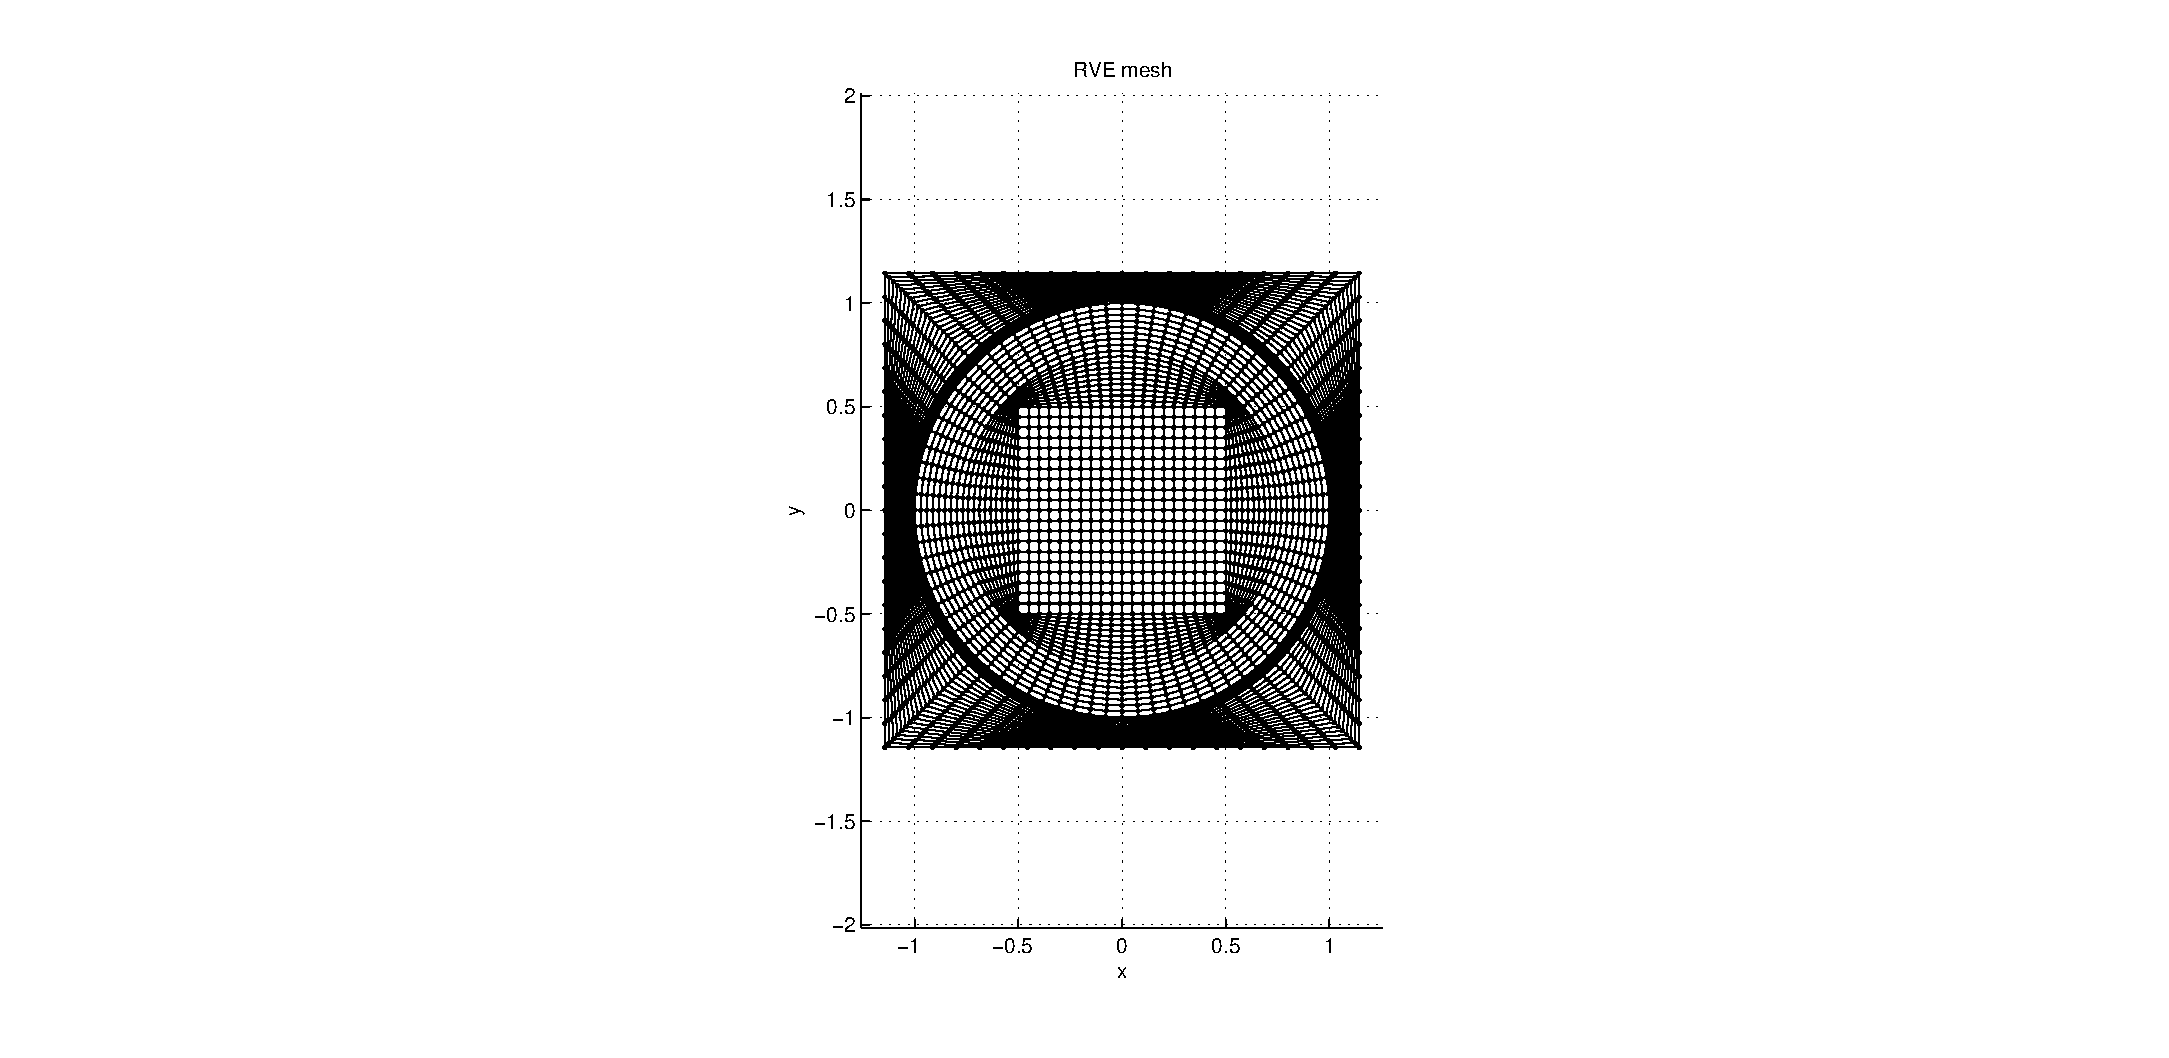
\includegraphics[width=0.95\textwidth]{mesh_single_order1}
  \end{figure} 
\end{frame}

\begin{frame}[t]
\frametitle{The result}
\vspace{-0.25cm}
 \centering
 \begin{figure}[!h]
  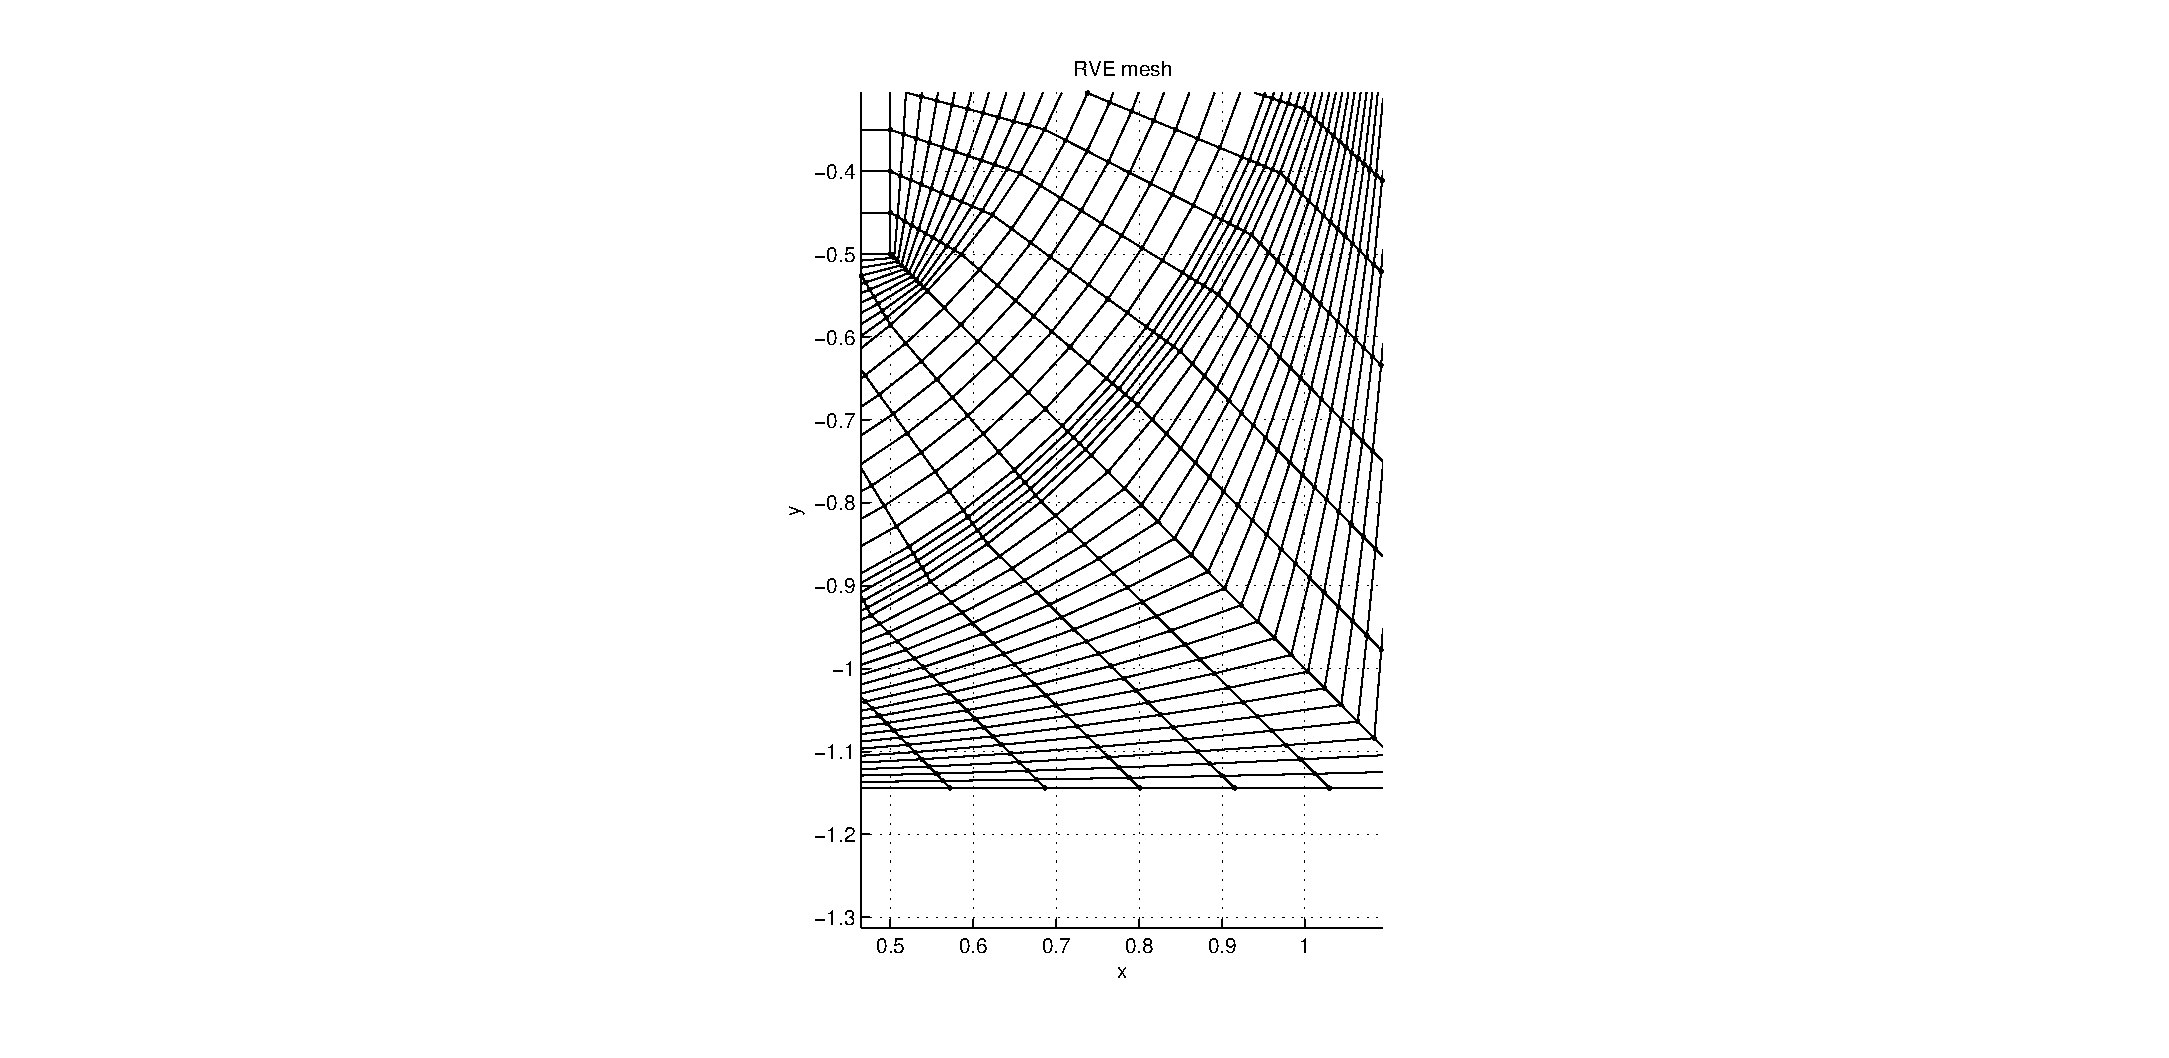
\includegraphics[width=0.95\textwidth]{mesh_single_order1-zoom1}
  \end{figure} 
\end{frame}

\subsection{Mesh generation algorithms}

\begin{frame}[t]
\frametitle{Fundamental ideas}
\vspace{-0.25cm}
 \centering
 \textit{One-to-one mapping}
 \begin{figure}[!h]
  \captionsetup[subfigure]{labelformat=empty}
   \centering
    \subfloat[][Computational domain]{\includegraphics[width=0.39\textwidth]{LBM_3D_surf.png}}
    \hspace{.1mm}
 \subfloat[][]{\includegraphics[width=0.2\textwidth]{arrow.png}}
    \hspace{.1mm}
    \subfloat[][Physical domain]{\includegraphics[width=0.39\textwidth]{curviLBM_3D_surf.png}}
  \end{figure} 
\end{frame}

\begin{frame}[t]
\frametitle{Fundamental ideas}
\vspace{-0.3cm}
\centering
 \textit{Helical numbering}
{\footnotesize
\begin{itemize}
\item $N_{1}$, $N_{2}$, $N_{3}$ number of grid points respectively along $\xi-$, $\eta-$, $\zeta-$ direction in computational space
\item Total number of points $N=N_{1}\cdotp N_{2}$ in 2D and $N=N_{1}\cdotp N_{2}\cdotp N_{3}$ in 3D
\item Helical numbering: given $n\in[1,N]$, $i\in[1,N_{1}]$, $j\in[1,N_{2}]$, $k\in[1,N_{3}]$, $n=i+(j-1)\cdotp N_{1}$ in 2D and $n=i+(j-1)\cdotp N_{1}+(k-1)\cdotp N_{1}\cdotp N_{2}$ in 3D
\end{itemize}
}
\vspace{-0.25cm}
 \begin{figure}[!h]
  \captionsetup[subfigure]{labelformat=empty}
   \centering
    \subfloat[][]{\includegraphics[height=0.45\textheight]{helical_num_2D.png}}
    \hspace{1cm}
    \subfloat[][]{\includegraphics[height=0.45\textheight]{helical_num_3D.png}}\\
  \end{figure} 
\end{frame}

\begin{frame}[label=3D_gen]
\frametitle{Mesh generation}
\vspace{-0.15cm}
\centering
{\footnotesize
\textit{Numerical strategy for structured grid generation in curved geometries - }}
{\scriptsize
\textit{3D (\hyperlink{2D_gen}{\beamerbutton{2D}})}
%\textit{3D}
\vspace{0.15cm}
\begin{enumerate}
\item The boundary is generated patching analytical parameterizations
\item The boundary is split into a set of 8 corners ($c_{i}$), 12 edges ($e_{i}$), 4 surfaces ($f_{i}$)
\item Interior nodes are created applying transfinite interpolation using multi-dimensional linear Lagrangian or Hermite interpolants
\begin{equation*}
P_{1}(x,p_{j})=\sum_{j=1}^{n}p_{j}\prod_{k=1,\ k\neq j}^{n}\frac{x-x_{k}}{x_{j}-x_{k}}
\end{equation*}
\begin{equation*}
P_{2}(x,y,p_{j},q_{j})=P_{1}(x,p_{j})\otimes P_{1}(y,q_{j})\quad P_{3}(x,y,z,p_{j},q_{j},r_{j})=P_{1}(x,p_{j})\otimes P_{1}(y,q_{j})\otimes P_{1}(z,r_{j})
\end{equation*}
\begin{equation*}
\begin{split}
r_{i}(\xi,\eta,\zeta)&=P_{1}(\xi,f_{5},f_{3})+P_{1}(\eta,f_{2},f_{4})+P_{1}(\zeta,f_{1},f_{6})- P_{2}(\xi,\eta,c_{1},c_{2},c_{3},c_{4})+\\&- P_{2}(\xi,\eta,e_{5},e_{6},e_{7},e_{8})- P_{2}(\xi,\zeta,e_{2},e_{4},e_{10},e_{12})- P_{2}(\eta,\zeta,e_{1},e_{3},e_{9},e_{11})+\\&+P_{3}(\xi,\eta,\zeta,c_{1},c_{2},c_{3},c_{4},c_{5},c_{6},c_{7},c_{8})
\end{split}
\end{equation*}
\item The mesh is smoothed applying elliptic mesh generation
\begin{equation*}
g^{11}\underline{r}_{,\xi\xi}+2g^{12}\underline{r}_{,\xi\eta}+g^{22}\underline{r}_{,\eta\eta}+2g^{13}\underline{r}_{,\xi\zeta}+g^{33}\underline{r}_{,\zeta\zeta}+2g^{23}\underline{r}_{,\eta\zeta}=0
\end{equation*}
\end{enumerate}
}
\end{frame}

% \begin{frame}[t]
% \frametitle{Geometry and mesh generation}
% \vspace{-0.5cm}
% \centering
% \textit{Numerical strategy for internal and external flow geometries}
% \begin{figure}[!h]
%   \captionsetup[subfigure]{labelformat=empty}
%    \centering
%     \subfloat[][]{\includegraphics[width=0.45\textwidth]{ref_square.png}}
%     \hspace{.5mm}
%     \subfloat[][]{\includegraphics[width=0.45\textwidth]{ref_cube.png}}
%   \end{figure} 
% \end{frame}

\begin{frame}[label=linear_system]
\frametitle{Mesh generation}
\vspace{-0.4cm}
\centering
{\footnotesize
\textit{Numerical strategy for structured grid generation in curved geometries  \hyperlink{num_stra}{\beamerbutton{More}}}
}
\begin{itemize}
\item {\scriptsize For both transfinite interpolation and elliptic mesh generation, Dirichlet boundary conditions are assigned, i.e. boundaries are fixed}
\item {\scriptsize Elliptic mesh generation is solved iteratively: at step $n$, the contravariant metric components are computed based on configuration at step $n-1$ and afterwards the configuration is updated}
\item {\scriptsize Partial differential equations are discretized using second order central finite difference scheme for second derivatives:}
{\scriptsize
\begin{equation*}
\frac{\partial^{2} u}{\partial (q^{i})^{2}}|_{q^{i}}=\frac{u_{i+1}-2u_{i}+u_{i-1}}{(\Delta q^{i})^{2}}-\frac{(\Delta q^{i})^{2}}{12}\frac{\partial^{4} u}{\partial (q^{i})^{4}}|_{q^{i}}+\dots
\end{equation*}
}
{\scriptsize An algebraic system of equations $\underline{\underline{A}}\underline{x}=\underline{b}$ is obtained; it is solved using built-in libraries in Matlab, and implementing an iterative Jacobian-Free Newton-Krylov (JFNK) method in C++}
%{\scriptsize An algebraic system of equations is obtained $\underline{\underline{A}}\underline{x}=\underline{b}$ which is solved using suitable libraries/commands in C++/Matlab}
\item {\scriptsize Management of boundaries is done exclusively using indices, not using coordinates: indices of nodes on corners, edges, faces are stored at the beginning of computation}
\end{itemize}
\end{frame}

\subsection{Differential geometry algorithms}

\begin{frame}[t]
\frametitle{Differential geometry}
\vspace{-0.5cm}
\centering
\textit{\footnotesize Computation of geometric properties of mappings}
 \begin{figure}[!h]
  \captionsetup[subfigure]{labelformat=empty}
   \centering
    \subfloat[][]{\includegraphics[width=0.45\textwidth, height=0.45\textheight]{cov_vec_surf.png}}\qquad
    \subfloat[][]{\includegraphics[width=0.45\textwidth, height=0.45\textheight]{cov_vec_space.png}}
  \end{figure}
\vspace{-0.25cm}
  \begin{itemize}
  \item {\scriptsize Given analytical parameterization, using symbolic computing (Mathematica)}
  \item {\scriptsize Given discrete data, using numerical computing (Matlab, C++)}
  \item {\scriptsize For 2D and 3D geometries, surfaces in 3D space}
  \end{itemize}
\end{frame}

\begin{frame}[t]
\frametitle{Differential geometry}
\vspace{-0.1cm}
\centering
{\footnotesize
%\textit{How do we compute geometric properties (metric, curvature,\dots) of manifolds?}
%\vspace{0.25cm}
\begin{columns}
\begin{column}{0.5\textwidth}
\begin{equation*}
\underline{R}=r_{i}=r_{i}(q^{j})
\end{equation*}
\begin{equation*}
\underline{g}_{i}=\frac{\partial\underline{R}}{\partial q^{i}}
\end{equation*}
\begin{equation*}
\underline{g}_{3}=\underline{g}_{1}\times\underline{g}_{2}\quad\text{for surfaces}
\end{equation*}
\begin{equation*}
g_{ij}=\underline{g}_{i}\cdotp\underline{g}_{j}
\end{equation*}
\begin{equation*}
g=det(g_{ij})
\end{equation*}
\begin{equation*}
\underline{g}^{i}=\frac{\underline{g}_{j}\times\underline{g}_{k}}{\sqrt[]{g}}
\end{equation*}
\begin{equation*}
g^{ij}=\underline{g}^{i}\cdotp\underline{g}^{j}
\end{equation*}
\begin{equation*}
v_{i}=\underline{v}\cdotp\underline{g}_{i}\quad v^{i}=\underline{v}\cdotp\underline{g}^{i}
\end{equation*}
\end{column}
\begin{column}{0.5\textwidth}
\begin{equation*}
\underline{v}=\sum_{i}v_{i}\underline{g}^{i}\quad \underline{v}=\sum_{i}v^{i}\underline{g}_{i}
\end{equation*}
\begin{equation*}
[ij,k]=\underline{g}_{i,j}\cdotp\underline{g}_{k}
\end{equation*}
\begin{equation*}
\Gamma^{k}_{ij}=\underline{g}_{i,j}\cdotp\underline{g}^{k}
\end{equation*}
\begin{equation*}
R^{l}_{ijk}=\Gamma^{l}_{ik,j}-\Gamma^{l}_{ij,k}+\Gamma^{l}_{js}\Gamma^{s}_{ik}-\Gamma^{l}_{ks}\Gamma^{s}_{ij}
\end{equation*}
\begin{equation*}
R_{iklm}=g_{ls}R^{s}_{ijk}
\end{equation*}
\begin{equation*}
R_{ij}=g^{lm}R_{iljm}
\end{equation*}
\begin{equation*}
R=g^{ij}R_{ij}
\end{equation*}
\end{column}
\end{columns}
}
\end{frame}

\begin{frame}[label=diffgeom]
\frametitle{Differential geometry}
\vspace{-0.6cm}
\centering
%\textit{How do we compute geometric properties (metric, curvature,\dots) of manifolds?}
%\vspace{0.25cm}
\begin{columns}
\begin{column}{0.3\textwidth}
 \begin{figure}[!h]
  \captionsetup[subfigure]{labelformat=empty}
   \centering
    \subfloat[][]{\includegraphics[height=0.25\textheight]{FD_stencil_2D.png}}\\
    \vspace{.5mm}
    \subfloat[][]{\includegraphics[height=0.35\textheight]{FD_stencil_3D.png}}
  \end{figure}
    \vspace{-1cm}
\hyperlink{diffgeom_details}{\beamerbutton{Additional details}}
\end{column}
\begin{column}{0.7\textwidth}
{\scriptsize
\begin{itemize}
\item First derivatives computed with second order finite differences
\begin{equation*}
\frac{\partial u}{\partial q^{i}}|_{q^{i}}=\frac{u_{i+1}-u_{i-1}}{2\Delta q^{i}}-\frac{(\Delta q^{i})^{2}}{6}\frac{\partial^{3} u}{\partial (q^{i})^{3}}|_{q^{i}}+\dots
\end{equation*}
\item Right- and left- sided second order finite differences at boundary
\begin{equation*}
\frac{\partial u}{\partial q^{i}}|_{q^{i}}=\frac{-3u_{i}+4u_{i+1}-u_{i+2}}{2\Delta q^{i}}+\frac{(\Delta q^{i})^{2}}{3}\frac{\partial^{3} u}{\partial (q^{i})^{3}}|_{q^{i}}+\dots
\end{equation*}
\begin{equation*}
\frac{\partial u}{\partial q^{i}}|_{q^{i}}=\frac{3u_{i}-4u_{i-1}+u_{i-2}}{2\Delta q^{i}}+\frac{(\Delta q^{i})^{2}}{3}\frac{\partial^{3} u}{\partial (q^{i})^{3}}|_{q^{i}}+\dots
\end{equation*}
\item $\Delta q^{i}$ are assumed to be constant in space and time but could be different between different directions, as considered in the computational space
\end{itemize}
}
\end{column}
\end{columns}
\end{frame}

\begin{frame}[plain]
\frametitle{}
\vspace{1cm}
\centering
{\LARGE
\textsc{Thank you!}
}
\end{frame}

\section{Appendices}

\begin{frame}[label=diffgeom_matlab_details]
\frametitle{Differential geometry}
\vspace{-0.3cm}
\centering
\textit{Details on Matlab implementation}
\vspace{0.25cm}
\begin{itemize}
\item In array \textit{firstdevneighbours} of dimension $N\times4D$, neighbours and type of finite difference scheme (encoded with an integer mask, from 1 to 3) are stored for each grid site
\item Each geometric quantity is stored in array of dimension $N\times D^{n_{indices}}$; i.e. tensor components are stored in columns $N\times 1$ stacked together in a single global array
\item Symmetry of geometric quantities (for example, $g_{ij}=g_{ji}$) is exploited: components that can be recovered by symmetry are not saved to disk
\end{itemize}
{\raggedleft
Back to \hyperlink{diffgeom}{\beamerbutton{Differential geometry}}
}
\end{frame}

\begin{frame}[label=diffgeom_cpp_details]
\frametitle{Differential geometry}
\vspace{-0.3cm}
\centering
\textit{Details on C++ implementation}
\vspace{0.25cm}

{\raggedleft
Back to \hyperlink{diffgeom}{\beamerbutton{Differential geometry}}
}
\end{frame}

\begin{frame}[label=2D_gen]
\frametitle{Mesh generation}
\vspace{-0.25cm}
\centering
{\footnotesize
\textit{Numerical strategy for structured grid generation in curved geometries - }}
{\scriptsize
\textit{2D}
\vspace{0.1cm}
\begin{enumerate}
\item The boundary is generated patching analytical parameterizations
\item The boundary is split into a set of 4 corners ($c_{i}$) and 4 edges ($e_{i}$)
\item Interior nodes are created applying transfinite interpolation using multi-dimensional linear Lagrangian interpolants
\begin{equation*}
P_{1}(x,p_{j})=\sum_{j=1}^{n}p_{j}\prod_{k=1\ k\neq j}^{n}\frac{x-x_{k}}{x_{j}-x_{k}}\quad P_{2}(x,y,p_{j},q_{j})=P_{1}(x,p_{j})\otimes P_{1}(y,q_{j})
\end{equation*}
\begin{equation*}
r(\xi,\eta)=P_{1}(\xi,e_{2},e_{4})+P_{1}(\eta,e_{1},e_{3})- P_{2}(\xi,\eta,c_{1},c_{2},c_{3},c_{4})
\end{equation*}
\item The mesh is smoothed applying elliptic mesh generation
\begin{equation*}
g^{11}\underline{r}_{,\xi\xi}+2g^{12}\underline{r}_{,\xi\eta}+g^{22}\underline{r}_{,\eta\eta}=0
\end{equation*}
\end{enumerate}
Back to \hyperlink{3D_gen}{\beamerbutton{Mesh generation}}
}
\end{frame}
\begin{frame}[label=num_stra]
\frametitle{Geometry and mesh generation}
%\vspace{-0.5cm}
\centering
\textit{Numerical strategy for monolithic domains}
\vspace{0.1cm}
{\footnotesize
\begin{itemize}
\item Cells are indexed with the same criteria applied to nodes and can be accessed using look-up tables of such indices
\item 3D geometries can be costructed directly using 3D transfinite interpolation and 3D elliptic smoothing or can be generated as extrusion of 2D geometries
\item If needed, cells can be accessed and modified, i.e. creating triangles/tetrahedra instead of squares/cubes
\end{itemize}
}
{\small
\raggedleft
Back to \hyperlink{mesh2}{\beamerbutton{Mesh generation}}
}
\end{frame}

\begin{frame}[t]
\frametitle{Geometry and mesh generation}
%\vspace{-0.5cm}
\centering
\textit{Numerical strategy for domains with random inclusions}
\vspace{0.2cm}
{\footnotesize
\begin{itemize}
\item 2D and 3D Ising model is applied to generate a porous geometry, controlling the dimensions of structures through the 'temperature' of the sytem
\item Nodes with positive magnetization are assigned to one material domain and those negative to the other material (or viceversa)
\item Boundaries of the 2 domains are identified checking magnetization of neighbours
\item Both domains are then separately smoothed using elliptic mesh generation iterations
\end{itemize}
}
{\small
\raggedleft
Back to \hyperlink{mesh2}{\beamerbutton{Mesh generation}}
}
\end{frame}




%\section{References}

%\begin{frame}[t,label=references,allowframebreaks]
%       \frametitle{References}
%	\begin{itemize}
%%	\item Loading rate effects on delamination:\\[10pt] \textit{Loading\_rate\_effects\_on\_CFRP.bib}\\[30pt]
%	\item Body-fitted grids for FSI modeling with LBM:\\[10pt] %\textit{Fluid\_structure\_interaction\_on\_deformable\_surfaces.bib}
%	\end{itemize}
%        \bibliographystyle{amsalpha}
%        {\footnotesize
%          \bibliography{PSI_talk.bib}
%        }
        %\bibliography{/auto.mounter/home/lucadistasio/Documents/ETH/Research_material/References/fsi_references_kbib.bib}
%\end{frame}

\begin{frame}[plain]
\frametitle{}
\end{frame}

\end{document}
